\chapter{Implementation} \label{chap:impl}
The prototype was created with Unity, which is Microsoft's recommended engine for creating HoloLens applications. Coding was done in C\# using Visual Studio. The project included the \textit{MixedRealityToolkit} \cite{Microsof99:online}, a collection of commonly used scripts and components for creating mixed reality applications, provided by Microsoft themselves. Using this package, setting up a HoloLens project is fairly straightforward, and functionality like gesture control and spatial mapping is quick to implement. We also included Vuforia, a popular AR framework, for its ability to recognize markers in the real world and anchor virtual objects to them.



\begin{figure}
    \centering
    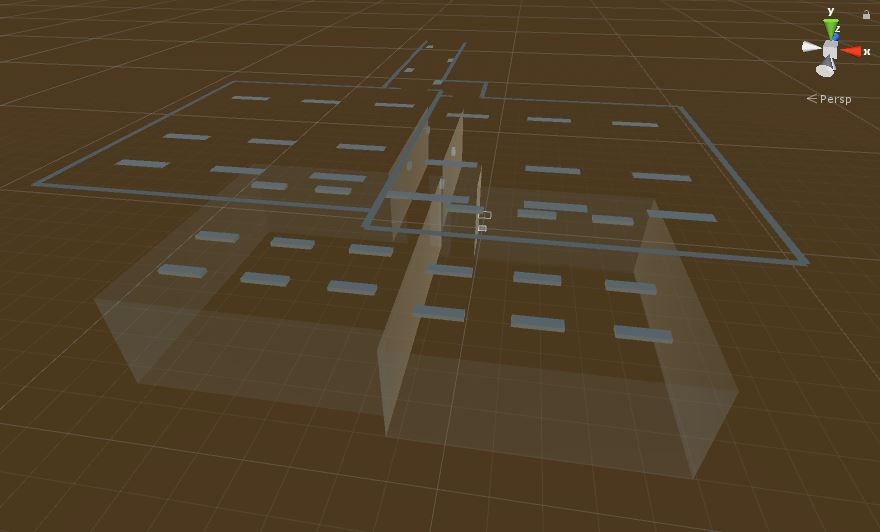
\includegraphics[width=1.0\linewidth]{resources/implementation/model.jpg}
    \caption{View of the scene in the Unity editor.}
    \label{fig:model}
\end{figure}

- Mapping of the workplace

- Implementation of lights, switches and circuits

- Implementation of minimap

- Usage of Vuforia for calibration

- Several paragraphs on the different visualizations

- Remote control of the visualizations
